\documentclass[12pt]{article}

\usepackage[utf8]{inputenc}

% graphics
\usepackage{graphicx}
\usepackage[pdf]{graphviz}
\usepackage{amsmath}
\usepackage{amsfonts}
\usepackage{amssymb}
\usepackage{amsthm}
\usepackage{algorithm}
\usepackage{algpseudocode}
\usepackage{titling}
\usepackage{listings}
\usepackage{tikz}
\usetikzlibrary{automata,arrows,positioning,calc}



% citation
\usepackage{biblatex}
\addbibresource{report.bib}

% MACROS
\newcommand*{\QED}{\hfill\ensuremath{\square}}
\newcommand{\stirlingii}{\genfrac{\{}{\}}{0pt}{}}

\theoremstyle{definition}
\newtheorem{definition}{Definition}[section]

\newtheorem{theorem}{Theorem}
\newtheorem{lemma}[theorem]{Lemma}

\newcommand{\subtitle}[1]{%
  \posttitle{%
    \par\end{center}
  \begin{center}\large#1\end{center}
  \vskip0.5em}%
}

\newcommand*{\oh}{\frac{1}{2}}
% title
\title{Bayesian parameter synthesis of Markov population models}
\subtitle{Master Project on Modeling of Complex, Self-organizing systems}
\author{Huy Phung\\University of Konstanz}
\date{\today}

\setlength{\headheight}{23pt}
\setlength{\parindent}{0.0in}
\setlength{\parskip}{0.0in}


\begin{document}
\maketitle
\pagebreak
\tableofcontents
\pagebreak

\begin{abstract}
  We study the collective behavior of a bee colony. Each bee in a colony could
  sting after observing a threat in the surrounding environment, and warn other
  bees by releasing a special substance, pheromone. By sensing the pheromone
  released in the environment, other bees in the colony may also sting. However,
  since stinging leads to the termination of an individual bee, it reduces the
  total defense capability as well. The stinging behavior of bee colonies can be
  studied by observing the changes in the bee population. In this project, we
  use parametric Markov Chain to model the bee population. The contributions of
  this project are (1) to show that steady-state distribution can be more
  precisely estimated with fewer data using Bayesian inference, and (2) Bayesian
  inference can also be used to estimate model parameters of parametric Markov
  Chain with more scalability (lower computational cost for models with a higher
  number of parameters, compare with the existing method with frequentist
  approach).
\end{abstract}

\section{Preliminaries}
\subsection{Discrete time Markov Chain}
Assume that each bee in a colony decides its next action (to sting or not to
sting) based only on the current state of the environment, and the number of
bees who sting or not sting can be modeled as a Markov process. To reduce the
complexity of the model, we make another assumption that the observations on a
bee colony are conducted in uniform time duration, hence the model is of
discrete-time. Therefore, Discrete-Time Markov Chain is the selected
mathematical model to describe the bee colony population. The definitions and
notations on this section are based on \cite{baier2008principles} and \cite{hajnal2019data}

\begin{definition}[Discrete Time Markov Chain]
  A Discrete Time Markov Chain (DTMC) is a tuple $(S,\mathbf{P}, S_{init}, AP,
  L)$
  \begin{itemize}
  \item $S$ is a countable nonemty set of \textit{states}
  \item $\mathbf{P}:S\times S \rightarrow [0,1]$ is the \textit{transition probability}
    function, s.t $$\sum_{s'\in S}\mathbf{P}(s, s') = 1$$
  \item $S_{init}: S \rightarrow [0,1]$ is the \textit{initial distribution},
    s.t  $$\sum_{s'\in S}S_{init}(s') = 1$$
  \item $AP$ is a set of \textit{atomic propositions}
  \item $L: S \rightarrow 2^{AP}$ is the labelling function on states.
  \end{itemize}
\end{definition}

The transition probability function in DTMC is given as a stochastic matrix $\mathbf{P}$,
that is, $\mathbf{P}$ satisfies the following properties
\begin{itemize}
\item $\mathbf{P}$ is a square matrix.
\item all elements are in $[0,1]$.
\item row elements sum up to 1.
\end{itemize}

Given a model $\mathcal{M}$, the population in steady state is represented by a
set of special states, namely \textit{terminal Strongly Connected Components}
\begin{definition}[Terminal Strongly Connected Components]
  Let $\mathcal{M}= (S,\mathbf{P}, S_{init}, AP, L)$ a DTMC, a state $s\in
  S$ is a Terminal Strongly Connected Component (tSCC for short) if and only if
  $P(s, s) = 1$ and $P(s, s') = 0 \forall s' \in S, s' \neq s$
\end{definition}

In order to generalize the stochastic matrix to encompass unknown information of
the system, we introduce \textit{parametric DTMC}. Let $\theta =
(\theta_1,\ldots,\theta_n) \in [0,1]^n$, we represent each element in matrix
$\mathbf{P}$ as a polynomial function of $\theta$. Let $\mathbf{Pol}_\theta$ be the
set of polynomials $P: [0,1]^n \rightarrow [0,1]$. We define
\textit{parametric Discrete-Time Markov Chain}, or \textit{pMC} for short, as
follow:

\begin{definition}[Parametric DTMC]
  A parametric Discrete Time Markov Chain (pMC for short) is a tuple $(S,\theta,
  \mathbf{P}_\theta, S_{init}, AP,
  L)$
  \begin{itemize}
  \item $S$ is a countable nonemty set of \textit{states}
  \item $\theta$ is the set of model parameters
  \item $\mathbf{P}:S \times S \rightarrow \mathbf{Pol}_\theta$ is the \textit{transition probability}
    function that map a transition relation between two states to a polynomial
    function of $\theta$
  \item $S_{init}: S \rightarrow [0,1]$ is the \textit{initial distribution},
    s.t  $$\sum_{s'\in S}S_{init}(s') = 1$$
  \item $AP$ is a set of \textit{atomic propositions}
  \item $L: S \rightarrow 2^{AP}$ is the labelling function on states.
  \end{itemize}
\end{definition}
A concrete assignment of $\theta$ on pMC induces a DTMC. Let $\phi$ be a
specification on a pMC $\mathcal{M}$ (for example, in this project $\phi$ is the
steady-state distribution), we estimate the model parameter $\theta$, such that
$\mathcal{M} \models \phi$


\subsection{Bayesian inference}
\subsubsection{Bayesian parameter estimation}
Let $D$ be observed data. In statistical inference, we assume that the observed
data has a probability distribution of unknown parameter $\theta$, i.e
$D \sim P(D|\theta)$. In frequentist approach, the estimation
of $\theta$ based on long-run property, that is, given a large enough sample
size, expected value of parameter estimation $\hat{\theta}$ is equal to
$\theta$. Therefore, frequentist approach requires to gather a large amount of
data to deliver a close estimation $\hat{\theta}$. In Bayesian approach, we
reuse the information \textit{beliefs} gained from observed data to enhance the
accuracy of the estimation of $\hat{\theta}$. The main advantage of Bayesian
approach over frequentist approach is that it require less data to obtain an
estimation $\hat{\theta}$.\\
The beliefs obtained from prior knowledge of model parameter $\theta$ is
represented by \textit{prior
  distribution} $\pi(\theta)$.\\
Also, we have probability distribution of observed data, given parameter
$\theta$, $P(D|\theta)$. This is also called \textit{likelihood function}.\\
With Bayesian formula, we have
\begin{align*}
  \pi(\theta | D) = \frac{P(D|\theta)\pi(\theta)}{\int_\theta P(D|\theta)\pi(\theta)d\theta}
\end{align*}
$\int_\theta P(D|\theta)\pi(\theta)d\theta$ is called \textit{marginal
  distribution}. $\pi(\theta | D)$ is called \textit{posterior distribution}.
Computing posterior distribution is the essential part of Bayesian inference,
since it gives us the estimation of parameter $\theta$.

\subsubsection{Posterior conjugation}
Conjugated posteriors are special cases of Bayesian inference, in which the
prior and posterior distribution belongs to the same family of distribution.
Conjugated posteriors give us significant benefits
\begin{enumerate}
\item Tractability: we have analytical form of posterior distribution.
\item Computationally effective: updating model parameter is of linear time to
  the dimension of parameter.
\end{enumerate}
We consider two conjugated posterior: Binomial-Beta and Dirichlet-Multinomial
\begin{lemma}[Binomial-Beta Conjugation]
  Binomial distribution is conjugated to beta distribution.
\end{lemma}
\begin{proof}
  The observed data $D=(x_1,\ldots,x_n)$ is sampled from $Binomial(k, \theta)$ function
  \begin{align*}
    P(D|\theta) = \prod_{i=1}^n{k\choose x_i}\theta^{x_i}(1-\theta)^{k-x_i}
  \end{align*}
  The parameter $\theta$ is of $Beta(\alpha, \beta)$ distribution
  \begin{align*}
    \pi(\theta) = \theta^{\alpha-1}(1-\theta)^{\beta -1}
  \end{align*}
  We obtained:
  \begin{align*}
    \pi(\theta|D) &\sim P(D|\theta)\pi(\theta) \\
                  &\sim \theta^{\sum_{i=1}^n x_i}(1-\theta)^{nk -\sum_{i=1}^n x_i} \theta^{\alpha -1} (1-\theta)^{\beta-1} \\
                  &= \theta^{\alpha - 1 + \sum_{i=1}^n x_i}(1-\theta)^{\beta - 1 + nk -\sum_{i=1}^n x_i}
  \end{align*}
  Thus, the posterior is $Beta(\alpha + \sum_{i=1}^n x_i, \beta + nk -\sum_{i=1}^n x_i)$
\end{proof}
Generalize this conjugation, we also have Multinomial-Dirichlet conjugation.
\begin{lemma}[Multinomial-Dirichlet Conjugation]
  Multinomial distribution is conjugated to Dirichlet distribution.
\end{lemma}
\begin{proof}
  The observed data $D=(x_1,\ldots,x_n)$ is sampled from $Multinomial(n; \theta_1,\ldots,\theta_n)$ function
  \begin{align*}
    P(x_1,\ldots,x_n | N, \theta_0,\ldots,\theta_n) &= \frac{n!}{x_1!\ldots x_n!} \prod_{i=1}^n\theta_i^{x_i}
  \end{align*}
  The parameter $(\theta_1,\ldots,\theta_n)$ is
  $Dirichlet(\alpha_1,\ldots,\alpha_n)$
  \begin{align*}
    \pi(\theta_1,\ldots,\theta_n) = \frac{1}{\mathbf{B}(\alpha_1,\ldots,\alpha_n)}\prod_{i=1}^n\theta_i^{\alpha_i - 1}
  \end{align*}
  We obtain
  \begin{align*}
    \pi(\theta_1,\ldots,\theta_n|D) &\sim P(D|\theta)\pi(\theta) \\
                                    &\sim \prod_{i=1}^n\theta_i^{x_i} \prod_{i=1}^n\theta_i^{\alpha_i - 1} \\
                                    &\sim \prod_{i=1}^n\theta_i^{\alpha_i - 1 + \sum_{i=1}^n x_i}
  \end{align*}
  Thus, the posterior is $Dirichlet(\alpha_1 +  x_1,\ldots,\alpha_n
  +  x_n)$
\end{proof}
More detailed description in these cases can be found in \cite{tu2014dirichlet}
and \cite{baron2019probability}. We summarize the necessary results in the following table:
\begin{table}[]
\begin{tabular}{lllll}
\cline{1-3}
\multicolumn{1}{|l|}{Likelihood} & \multicolumn{1}{l|}{Prior} & \multicolumn{1}{l|}{Posterior parameters} &  &  \\ \cline{1-3}
  \multicolumn{1}{|l|}{$Binomial(k, \theta)$}  & \multicolumn{1}{l|}{$Beta(\alpha, \beta)$}  & \multicolumn{1}{l|}{$\alpha' = \alpha + \sum_{i=1}^n x_i, \beta' = \beta + nk -\sum_{i=1}^n x_i$}  &  &  \\ \cline{1-3}
  \multicolumn{1}{|l|}{$Multinomial(n; \theta_1,\ldots,\theta_n)$}  & \multicolumn{1}{l|}{$Dirichlet(\alpha_1,\ldots,\alpha_n)$}  & \multicolumn{1}{l|}{$\alpha_i' =\alpha_i + x_i, 1 \leq i \leq n$}  &  &  \\ \cline{1-3}
                        &                        &                        &  & 
\end{tabular}
\end{table}

\subsubsection{Markov Chain Monte Carlo method}
In case the posterior distribution has no analytical form or its analytical form
is difficult to sample from directly, we need to use
\textit{Metropolis-Hastings} algorithm (MH in short). The reason of using MH
algorithm to MH algorithm can draw samples from posterior distribution with only
the likelihood function. Using the MH algorithm, we can estimate the parameter
by posterior mean, without knowing the analytical form of posterior distribution
itself.

\begin{algorithm}[H]
  \caption{Metropolis-Hastings Algorithm, $D$ is the observation data, $\theta$ is parameter}\label{mhalg}
  \begin{algorithmic}[1]
    \Procedure{Metropolis-Hastings}{$D$, maxIteration}
    \State Select a proposal distribution $\pi(\theta)$
    \State Initialize $\theta$
    \While{maxIteration not reached}
    \State $L \leftarrow P(D|\theta)$
    \State Draw $\theta' $ from the proposal distribution (transition kernel).
    \State $L' \leftarrow P(D|\theta')$
    \If{ $\ln(L') - \ln(L) > 0$ }
    \State  $\theta = \theta'$ (accept $\theta'$)
    \Else
    \State with probability $\epsilon$ accept $\theta'$ (avoiding local maxima)
    \EndIf
    \EndWhile
    \EndProcedure
  \end{algorithmic}
\end{algorithm}
The likelihood function can be implemented as log-likelihood to avoid underflow
error. Proposal distribution defines how do we proceed to the next parameter
value on the parameter space; it can be of any distribution family. In this
project,
since parameters are in $[0,1]$, we select Beta distribution as proposal.\\
There are different methods to select the initial value of parameter $P$. In
this project, we initialize $P$ randomly. There are two advantages of using
Markov Chain Monte Carlo in Bayesian inference:
\begin{enumerate}
\item Parameter transition only needs the computation of likelihood function.
  Therefore, Monte Carlo Markov Chain can be used in general Bayesian inference,
  in which we are not guaranteed to have an analytical form of posterior.
\item Specifically in Metropolis-Hastings algorithm, marginal distribution is
  cancelled out, thus make MH a computationally efficient algorithm.
\end{enumerate}
However, MH algorithm also has a drawback; its convergence becomes slower as the
dimension of parameter $\theta$ increases.

\subsubsection{Bayesian Parameter Estimation}
With posterior distribution $\pi(\theta|D)$ we estimate the parameter
$\hat{\theta}$ using Bayesian posterior mean:
\begin{align*}
  \hat{\theta} = \mathbf{E}[\theta] = \int_\theta \theta \pi(\theta|D) d\theta
\end{align*}
In case we have samples from posterior distribution, for example when we use MH
algorithm, the discrete form of posterior mean is used:
\begin{align*}
  \hat{\theta} = \mathbf{E}[\theta] = \sum_\theta \theta \pi(\theta|D)
\end{align*}
\begin{definition}[Bayesian Credible Set]
  Set C is a $(1 − \alpha)100\%$ credible set for the parameter $\theta$ if the posterior
  probability for $\theta$ to belong to C equals $(1 − \alpha)$.
  \begin{align*}
    P(\theta \in C | D) = \int_C \pi(\theta|D) d\theta = 1 - \alpha
  \end{align*}
\end{definition}
In this project, we use $0.95$ credible set, i.e $\alpha=0.05$
\begin{definition}[Highest Posterior Density credible set]
  Highest Posterior Density $(1-\alpha)100\%$ credible set (HDP for short) is the
  interval with minimum length over all Bayesian $(1-\alpha)100\%$ Credible Set.
\end{definition}
In this project, the HPD is calculated using PyMC3 library
\cite{salvatier2016pymc3}

\section{Modeling of bees colony}
\subsection{Biological description}
We consider the collective action of a bee colony. Each bee in a colony could
possibly sting after observing a threat in the surrounding environment, and warn
other bees by releasing pheromone. By sensing the pheromone released in the
environment, other bees in the colony may also sting. Since stinging leads to
the termination of an individual bee, it reduces the total defense capability as
well. We studies how the actions of a bee changes with regarding to its
surrounding the environment. There are 3 assumptions on the system:
\begin{enumerate}
\item Each bee release an unit amount of pheromone immediately after stinging.
\item A bee dies after stinging and releasing pheromone. In the other words, no
  bee can sting more than once.
\item Stinging behaviour only depends on the concentration of pheromone in the
  environment.
\end{enumerate}
Under these assumption, a bee colony can be viewed as a set of agents (bees)
interact with each other in a closed environment with the appearance of a factor
\textit{pheromone}. Each agent in the colony observe the following two factors
of the environment: (1) amount of pheromone and (2) number of other agents.
Afterward, the agent has probability to commit an action, namely \textit{sting}.
The agent is eliminated from environment after stinging.

\subsection{Markov population models for bee colony}
Semantics of Markov population models for bees colony are developed by
\cite{hajnal2019data}. In this report we summarize three models of bees population
\begin{enumerate}
\item Synchronous model
\item Asynchronous model
\item Semi-synchronous model
\end{enumerate}
In the scope of this project we do not analyze the semantics of each model.
Instead, the inference methods presented only uses the polynomial function of
the models' steady-state distribution. 

\subsubsection*{Asynchronous model}
In asynchronous experiment we assume that there is almost improbable for two
bees to sting simultaneously, and any bees release pheromone immediately after
its death. By that observation we can assume that each bee
sting at different level of pheromone.\\
\begin{figure}[H]
  \centering 
  \begin{tikzpicture}[->, >=stealth', auto, semithick, node distance=3cm]
    \tikzstyle{every state}=[fill=white,draw=black,thick,text=black,scale=1]
    \node[state]    (A)                     {init};
    \node[state]    (B)[above right of=A]   {$\oh$};
    \node[state]    (C)[below right of=A]   {$1$};
    \node[state]    (D)[above right of=B]   {$\oh \oh$};
    \node[state]    (E)[below of=D]         {$\oh 1$};
    \node[state]    (F)[below of=E]         {$1 1$};
    \node[state]    (G)[above right of=D]   {$\oh \oh \oh$};
    \node[state]    (H)[below of=G]         {$\oh \oh 1$};
    \node[state]    (I)[below of=H]         {$\oh 1 1$};
    \node[state]    (J)[below of=I]         {$1 1 1$};
    \node[state]    (K)[right of=H]         {$0 \oh 1$};
    \node[state]    (L)[right of=I]         {$0 1 1$};
    \node[state]    (M)[right of=K]         {$0 0 1$};
    \path
    (A) edge node{$1-p$} (B)
    edge node{$p$} (C)
    (B) edge node{$1-p$} (D)
    edge node{$p$} (E)
    (C) edge node{$1-p$} (E)
    edge node{$p$} (F)
    (D) edge node{$1-p$} (G)
    edge node{$p$} (H)
    (E) edge node{$1-p$} (H)
    edge node{$p$} (I)
    (F) edge node{$1-p$} (I)
    edge node{$p$} (J)
    (H) edge node{$1-q$} (K)
    edge node{$q$} (I)
    (I) edge node{$1-q$} (L)
    edge node{$p$} (J)
    (K) edge node{$1-q$} (M)
    edge node{$p$} (L);
  \end{tikzpicture}
  \caption{Example asynchronous model of 3 bees, 2 parameters}
\end{figure}


\subsubsection*{Synchronous model}
In \textit{fully synchronous} experiment we assume that the number of stinging
bees is only counted after a fixed amount of time, so that without loss of
generality we can assume the pheromone diffuse almost immediately among the bee
colony, and each bee decide to sting or not to sting immediately after sensing
the pheromone concentration.\\

\begin{figure}[H]
  \centering 
\begin{tikzpicture}[->, >=stealth', auto, semithick, node distance=3cm]
\tikzstyle{every state}=[fill=white,draw=black,thick,text=black,scale=1]
\node[state]    (A)                     {init};
\node[state]    (B)[right of=A]         {$\oh \oh 1 $};
\node[state]    (C)[above of=B]         {$\oh \oh \oh$};
\node[state]    (D)[below of=B]         {$\oh 1 1$};
\node[state]    (E)[below of=D]         {$1 1 1$};
\node[state]    (F)[right of=B]         {$0 0 1$};
\node[state]    (G)[right of=D]         {$0 1 1$};
\path
(A) edge    node{$(1-p)^3$}        (B)
    edge    node{$(3p(1-p)^2$}     (C)
    edge    node{$3p(1-p)^2$}      (D)
    edge    node{$p^3$}            (E)
(B) edge    node{$(1-q)^2$}        (F)
    edge    node{$(2q(1-q)$}       (G)
    edge[bend left,below]    node{$q^2$}            (E)
(D) edge    node{$(1-q)$}          (G)
    edge    node{$q$}              (E); 
  \end{tikzpicture}
  \caption{Example synchronous model of 3 bees, 2 parameters.}
\end{figure}



\subsubsection*{Semi-synchronous model}
In \textit{Semisynchronous model}, we assume that the behaviour is initally
synchronous. That means, at the initial states we do synchronous update. From
all succeeding states from initial states, the updates are of asynchronous semantics.
\begin{figure}[H]
  \centering 
  \begin{tikzpicture}[->, >=stealth', auto, semithick, node distance=3cm]
    \tikzstyle{every state}=[fill=white,draw=black,thick,text=black,scale=1]
    \node[state]    (A)                     {init};
    \node[state]    (B)[right of=A]         {$\oh \oh 1 $};
    \node[state]    (C)[above of=B]         {$\oh \oh \oh$};
    \node[state]    (D)[below of=B]         {$\oh 1 1$};
    \node[state]    (E)[below of=D]         {$1 1 1$};
    \node[state]    (F)[right of=B]         {$0 \oh 1$};
    \node[state]    (G)[right of=D]         {$0 1 1$};
    \node[state]    (H)[right of=F]         {$0 1 1$};
    \path
(A) edge    node{$(1-p)^3$}        (B)
    edge    node{$(3p(1-p)^2$}     (C)
    edge    node{$3p(1-p)^2$}      (D)
    edge    node{$p^3$}            (E)
(B) edge    node{$1-q$}            (F)
    edge    node{$q$}              (D)
(D) edge    node{$(1-q)$}          (G)
    edge    node{$q$}              (E)
(F) edge    node{$q$}              (G)
    edge    node{$1 - q$}          (H);
  \end{tikzpicture}
  \caption{Example semisynchronous model of 3 bees, 2 parameters}
\end{figure}

For a population of $n$ bees, all three types of models share two properties:
\begin{enumerate}
\item Has exactly one initial state, $|S_{init}| = 1$. This assumption is
  obvious, since at the beginning of the experiment, all bees are alive.
\item Has $n+1$ tSCCs $(tSCC_0,\ldots,tSCC_n)$. This is because the number of
  dead bees cannot exceed the population size. It also follows that
  \begin{align*}
    \sum_{i=0}^n P(FG\quad tSCC_i) = 1
  \end{align*}
\end{enumerate}


\section{Bayesian parameter synthesis of Markov population model}
\subsection{Data}

Let $n$ be the population of bee in the colony. Assume that these $n$ bees are
in a closed environment, like a box. We use an initial stimulation, for example
threating the bees. Assume that all experiment have the same initial
stimulation, we observe how many bees are dead in the steady state. This
experiment has $n+1$ outcomes $0,1,\ldots,n$ dead bees.\\
Assume we conduct $N$ experiments, let $x_0,x_1,\ldots,x_N$ be the number of
dead bees. Since in each experiment, we have $(0 \leq x_1,\ldots,x_N \leq n+1)$,
we can place $x_i$ on $n+1$ bins from $0$ to $n$. Assume we model the system by
pMC $\mathcal{M}$ with steady-state distribution $\theta_0,\ldots,\theta_n$. Let
$a_i$ be the number of experiments which has outcome $i, 0 \leq i \leq n$, we
obtain that $a_i$ has \textit{multinomial distribution}:
\begin{align*}
  P(a_0,\ldots,a_n | N, \theta_0,\ldots,\theta_n) &\sim Multinomial(a_0,\ldots,a_n | N, \theta_0,\ldots,\theta_n) \\
                                                  &= \frac{n!}{a_0!\ldots a_n!} \theta_0^{a_0}\ldots \theta_n^{a_n}
\end{align*}
We use the multinomial distribution as likelihood function (data model) in the
following Bayesian inferences.

\subsection{Inference of steady state distribution}
Using the Multinomial-Dirichlet conjugation, we can infer the steady state
distribution as we observe new experiment data $D=(a_0,\ldots,a_n)$, with $a_i$
is the number of experiment in which the population in steady-state is $i$ 
\begin{algorithm}[H]
  \caption{Estimation of steady-state distribution given a sample $S$}\label{exp_a}
  \begin{algorithmic}[1]
    \Procedure{Estimate $p_i = P(tSCC_i)$}{$S$}
    \State Initialize $\alpha_0=\alpha_1=\ldots=\alpha_n=1$
    \State Initialize $p_0=p_1=\ldots=p_n=0$
    \State Update $\alpha_i = \alpha_i + a_i, 1 \leq i \leq n$
    \State Update $p_i = \alpha_i + \sum_{i=1}^n \alpha_i, 1 \leq i \leq n$
    \EndProcedure
  \end{algorithmic}
\end{algorithm}

As later shown in the implementation with synthetic data, the Bayesian
estimation of steady-state distribution converges quickly to the true parameter
used for data synthesis. This method does not directly estimate the pMC
model parameters. However, it can support the parameter estimation presented
\cite{hajnal2019data} to estimate the model parameters with narrower credible
set.

\subsection{Inference of model parameters}
We can also use Bayesian inference to estimate pMC model parameters directly.
Given a pMC $\mathcal{M}$ with $\theta=(\theta_1,\ldots,\theta_k)$ as its model
parameters. Since $\theta_i \in [0,1]$, we can assume that $\theta_i$ are of
$Beta(\alpha, \beta)$ distribution. Note that $\alpha, \beta$ are
hyperparameters and must be selected manually. Also note that
$\theta_1,\ldots,\theta_k$ are not simplex, thus it is not possible to use
Dirichlet prior. \\
In this method, since there is no possible use of posterior conjugation, thus
the hyperparameters estimation is hard and not in the scope of this project. Let
$f_i = P (FG\quad tSCC_i)$ are polynomial functions of steady-state
distribution, we denote $\epsilon_i = f_i(\theta)$ as evaluations of the
polynomial function with a concrete assignment of $\theta$. The steady-state
distribution has then $Multinomial(N, \epsilon = (\epsilon_0,\ldots,\epsilon_n))$ with $N$
is the sample size of experiment data $D$. The posterior distribution has the
following form:
\begin{align*}
  \pi(\theta|D) \sim Multinomial(N, (\epsilon_0,\ldots,\epsilon_n))\pi(\theta_1)\ldots\pi(\theta_k)
\end{align*}
As the posterior $\pi(\theta|D)$ has no analytical form, we use
Metropolis-Hastings to sample from it.
\begin{algorithm}[H]
  \caption{Estimation of model parameters given a sample $D$}\label{exp_b}
  \begin{algorithmic}[1]
    \Procedure{Estimate $\theta$}{$S$}
    \State Select hyperparameter $\alpha, \beta$
    \State Select $Beta(\alpha, \beta)$ as proposal distribution (transition
    kernel) for $\theta_i, 1\leq i \leq n$
    \State Initialize $\theta$
    \While{maxIteration not reached}
    \State Evaluate $\epsilon = (f_0(\theta),\ldots,f_n(\theta))$
    \State $L \leftarrow Multinomial(D|\epsilon)$
    \State Draw $\theta'$ from the proposal distribution.
    \State Evaluate $\epsilon' = (f_0(\theta),\ldots,f_n(\theta))$
    \State $L' \leftarrow P(D|\epsilon')$
    \If{ $\ln(L') - \ln(L) > 0$ }
    \State  $\theta = \theta'$ (accept $\theta'$)
    \Else
    \State with probability $\epsilon$ accept $\theta'$ (avoiding local maxima)
    \EndIf
    \EndWhile
    \EndProcedure
  \end{algorithmic}
\end{algorithm}


\subsection{Accuracy measures}
In order to evaluate the accuracy of parameter point inference, we have to
select a distance measure from estimated parameter to true parameter. In this
project we use two measures:
\begin{definition}[RMSE]
  Let $\theta = (\theta_1,\ldots,\theta_n)$ and $\hat{\theta} =
  (\hat{\theta_1},\ldots,\hat{\theta_n})$ be vectors of $n$ real numbers, the
  Root Mean Square Error between $p$ and $\hat{p}$ is defined as follow:
  \begin{align*}
    RMSE(\theta, \hat{\theta}) = \sqrt{\frac{\sum_{i=1}^n{(\theta_i - \hat{\theta_i})}}{n}}
  \end{align*}
\end{definition}

\section{Implementation and results}
The Bayesian inference methods are implemented in Python 3 and tested in the
followin system configuration:
\begin{itemize}
\item Intel Core i5-8265U @ 1.60GHz
\item 16GB RAM
\item OpenSUSE Tumbleweed 20200427
\item Anaconda 3 2019.10 for linux x86\_64
\end{itemize}
The following experiment on Bayesian inference use synthetic data from
semi-synchronous models of 2, 5 and 10 bees (in order to compare the performance
with related work in \cite{hajnal2019data}).


\subsection{Data synthesis}
The data synthesis for $n$ bees population is conducted as follow:
\begin{itemize}
\item Select a pMC model $\mathcal{M}$ to model the population of . Let
  $\bar{p}=p_1,\ldots,p_n$ is the model parameter vector.
\item Assign a concrete value for $\bar{p}$, called $\bar{p}_{true}$
\item From $\mathcal{M}$, deliver the rational functions of $f_i(\bar{p}) =
  P(FG\quad tSCC_i)$, $0 \leq i \leq n$. (using PRISM Model Checker \cite{KNP11})
\item Evaluate concrete value $\theta_i = f_i(\bar{p}_{true})$
\item Draw sample $S$ from multinomial distribution $Multinomial(N,
  \theta=(\theta_0,\ldots,theta_n))$
\item $S$ is the synthetic result for the experiment 3.1
\end{itemize}

\begin{figure}[H]
  \centering
  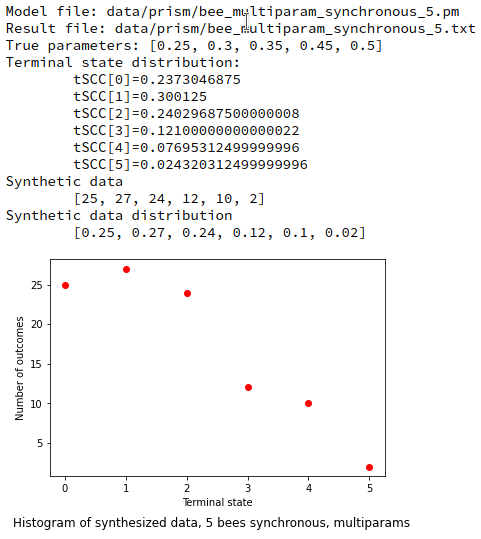
\includegraphics[width=0.6\textwidth,keepaspectratio]{figures/data_synthesis.png}
  \caption{Steady state data synthesis, semi-synchronous model of 5 bees
    population, model parameters $(0.3, 0.25, 0.35, 0.45, 0.5)$}
\end{figure}

\subsection{Inference of steady state distribution}
This experiment is conducted on semisynchronous model of 5 bees. The polynomial
functions of steady-state distribution is generated by PRISM and parsed into
Python 3 source code
(\texttt{semisync\_5bees.py}). The source code for this
experiment is on Jupyter Notebook file \texttt{visualization.ipynb}
\begin{figure}[H]
  \centering
  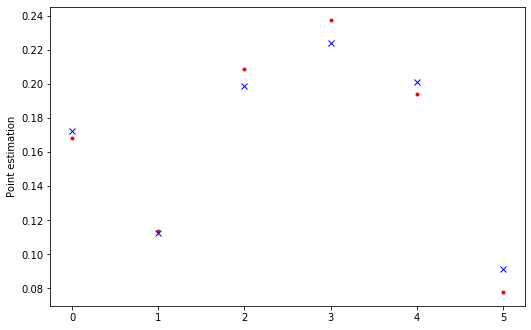
\includegraphics[width=0.6\textwidth,keepaspectratio]{figures/point_estimation.png}
  \caption{Bayesian estimation of steady state distribution}
\end{figure}
In order to compare with the work by \cite{hajnal2019data}, we also visualize
the interval calculated by the following formula:
\begin{align*}
  \theta_i \pm (z_{\alpha / 2}\sqrt{\frac{\theta_i(1-\theta_i)}{N}})
\end{align*}
where $N$ is the sample size. Experiment configurations:
\begin{itemize}
\item true model parameter: $[0.3, 0.25, 0.35, 0.45, 0.5]$
\item tSCC distribution evaluation: $[0.1680, 0.1139, 0.2089, 0.2371, 0.1940, 0.0778]$ 
\end{itemize}

\begin{figure}[H]
  \centering
  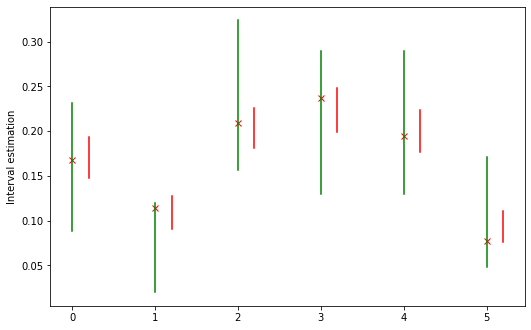
\includegraphics[width=0.6\textwidth,keepaspectratio]{figures/interval_estimation.png}
  \caption{Comparision of Bayesian Highest Posterior Density 95\% and interval
    estimated using method in \cite{hajnal2019data}}
\end{figure}


\subsection{Inference of model parameters}
This experiment is conducted in 2, 5, and 10 bees population models of 2, 5, and 10
parameters respectively. All models are semi-synchronous.\\
\begin{lstlisting}
  Experiment with 2 bees, 2 params, semisync
  Finished in 2.0310990789876087 seconds, chain length 50000
  True parameter: [0.1, 0.2]
  Estimated parameter: [0.10183236 0.18434951]
  RMSE: 0.00012414769020485024
  Log likelihood: -8.4331030579051
  AIC: 20.8662061158102

  Experiment with 5 bees, 5 params, semisync
  Finished in 7.2764098109910265 seconds, chain length 50000
  True parameter: [0.1, 0.2, 0.4, 0.5, 0.6]
  Estimated parameter: [
  0.10135125 0.21855681 0.52070207 0.45761621 0.57840823
  ]
  RMSE: 0.0034355521925440993
  Log likelihood: -70.33078101358842
  AIC: 150.66156202717684

  Experiment with 10 bees, 10 params, semisync
  Finished in 602.7453691669944 seconds, chain length 50000
  True parameter: [0.1, 0.2, 0.4, 0.5, 0.6, 0.1, 0.2, 0.4, 0.5, 0.6]
  Estimated parameter: [
  0.11375671 0.14925181 0.3042601  0.57028791 0.81435131
  0.10468808 0.37077345 0.40401714 0.28729648 0.28731649
  ]
  RMSE: 0.02350330802802734
  Log likelihood: -395.266357301065
  AIC: 810.53271460213

\end{lstlisting}

\subsection{Notes on implementation}
A script \texttt{parse\_prism.py} is include in folder \texttt{models} to parse
PRISM polynomial string to a Python class template. This is to avoid calling
expensive function \texttt{eval()} on runtime. Source code structure:
\begin{itemize}
\item \texttt{docs} folder contains final report
\item \texttt{impl} folder contains python implementation and PRISM results
  parsed to Python classes
\item \texttt{examples} folder contains jupyter notebook examples.
\end{itemize}

\section{Conclusion}
The goal of this project is to experiment Bayesian approach on parameter
inference of Markov population models. The results shows that Bayesian inference
is efficient to deliver an estimation of model parameters. Furthermore, the
implementation is more efficient than the work in \cite{hajnal2019data} as it
can work with higher number of parameters and requires less computational
resources.\\
However, there are still problems
\begin{enumerate}
\item MH algorithm converges slower as the number of parameter increases, thus
  requires longer chain of sampling the parameter space, which may increase the
  computational cost dramatically.
\item PRISM is still necessary to deliver polynomial functions, thus introduce
  an overhead, that PRISM itself is resource-hungry.
\item In this project, there is no Bayesian inference, which is designed to deal
  with the case when the polynomial functions are hard to synthesize, or
  impossible to synthesize.
\end{enumerate}
However, we believe that the method can be developed further to overcome these limitations.


\printbibliography

\end{document}


